
\documentclass[11pt]{article}
\usepackage[a4paper,margin=2.2cm]{geometry}
\usepackage{amsmath,amssymb,bm}
\usepackage{booktabs}
\usepackage{array}
\usepackage{xcolor}
\usepackage{tikz}
\usepackage{pgfplots}
\usepackage{hyperref}
\usepackage{enumitem}
\pgfplotsset{compat=1.18}
\usetikzlibrary{arrows.meta,positioning,calc,fit,matrix}

\definecolor{lowblue}{RGB}{225,240,255}
\definecolor{midblue}{RGB}{120,180,230}
\definecolor{highblue}{RGB}{15,90,160}
\definecolor{lowgreen}{RGB}{230,245,230}
\definecolor{midgreen}{RGB}{120,190,120}
\definecolor{highgreen}{RGB}{20,120,40}
\definecolor{loworange}{RGB}{255,240,220}
\definecolor{midorange}{RGB}{245,170,80}
\definecolor{highorange}{RGB}{190,80,20}
\definecolor{lowred}{RGB}{255,230,230}
\definecolor{midred}{RGB}{240,120,120}
\definecolor{highred}{RGB}{170,20,40}
\definecolor{purpleA}{RGB}{235,225,245}
\definecolor{purpleB}{RGB}{165,120,200}
\definecolor{purpleC}{RGB}{90,40,140}
\definecolor{clusterone}{RGB}{225,240,255}
\definecolor{clustertwo}{RGB}{255,230,190}
\definecolor{clusterthree}{RGB}{230,245,220}
\definecolor{clusterfour}{RGB}{245,220,245}

\newcommand{\cellbox}[2]{\fill[#1] #2 rectangle ++(0.8,0.8);}
\newcommand{\gridframe}{\draw[black!40,step=0.8] (0,0) grid (4,4);}
\newcommand{\rastlabel}[1]{\node[font=\scriptsize,align=center] at (2,-0.35) {#1};}

\newcommand{\drawRasterCOne}{%
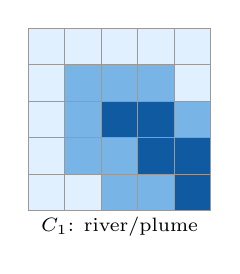
\begin{tikzpicture}[scale=0.58]
\cellbox{lowblue}{(0,0)} \cellbox{lowblue}{(0.8,0)} \cellbox{midblue}{(1.6,0)} \cellbox{midblue}{(2.4,0)} \cellbox{highblue}{(3.2,0)}
\cellbox{lowblue}{(0,0.8)} \cellbox{midblue}{(0.8,0.8)} \cellbox{midblue}{(1.6,0.8)} \cellbox{highblue}{(2.4,0.8)} \cellbox{highblue}{(3.2,0.8)}
\cellbox{lowblue}{(0,1.6)} \cellbox{midblue}{(0.8,1.6)} \cellbox{highblue}{(1.6,1.6)} \cellbox{highblue}{(2.4,1.6)} \cellbox{midblue}{(3.2,1.6)}
\cellbox{lowblue}{(0,2.4)} \cellbox{midblue}{(0.8,2.4)} \cellbox{midblue}{(1.6,2.4)} \cellbox{midblue}{(2.4,2.4)} \cellbox{lowblue}{(3.2,2.4)}
\cellbox{lowblue}{(0,3.2)} \cellbox{lowblue}{(0.8,3.2)} \cellbox{lowblue}{(1.6,3.2)} \cellbox{lowblue}{(2.4,3.2)} \cellbox{lowblue}{(3.2,3.2)}
\gridframe\rastlabel{$C_1$: river/plume}
\end{tikzpicture}}

\newcommand{\drawRasterCTwo}{%
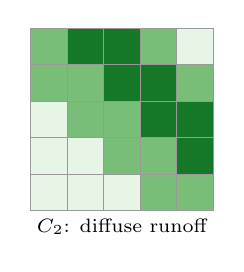
\begin{tikzpicture}[scale=0.58]
\cellbox{lowgreen}{(0,0)} \cellbox{lowgreen}{(0.8,0)} \cellbox{lowgreen}{(1.6,0)} \cellbox{midgreen}{(2.4,0)} \cellbox{midgreen}{(3.2,0)}
\cellbox{lowgreen}{(0,0.8)} \cellbox{lowgreen}{(0.8,0.8)} \cellbox{midgreen}{(1.6,0.8)} \cellbox{midgreen}{(2.4,0.8)} \cellbox{highgreen}{(3.2,0.8)}
\cellbox{lowgreen}{(0,1.6)} \cellbox{midgreen}{(0.8,1.6)} \cellbox{midgreen}{(1.6,1.6)} \cellbox{highgreen}{(2.4,1.6)} \cellbox{highgreen}{(3.2,1.6)}
\cellbox{midgreen}{(0,2.4)} \cellbox{midgreen}{(0.8,2.4)} \cellbox{highgreen}{(1.6,2.4)} \cellbox{highgreen}{(2.4,2.4)} \cellbox{midgreen}{(3.2,2.4)}
\cellbox{midgreen}{(0,3.2)} \cellbox{highgreen}{(0.8,3.2)} \cellbox{highgreen}{(1.6,3.2)} \cellbox{midgreen}{(2.4,3.2)} \cellbox{lowgreen}{(3.2,3.2)}
\gridframe\rastlabel{$C_2$: diffuse runoff}
\end{tikzpicture}}

\newcommand{\drawRasterCThree}{%
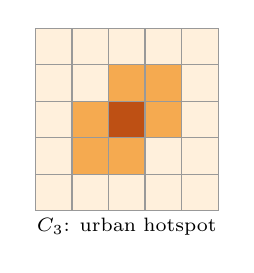
\begin{tikzpicture}[scale=0.58]
\cellbox{loworange}{(0,0)} \cellbox{loworange}{(0.8,0)} \cellbox{loworange}{(1.6,0)} \cellbox{loworange}{(2.4,0)} \cellbox{loworange}{(3.2,0)}
\cellbox{loworange}{(0,0.8)} \cellbox{midorange}{(0.8,0.8)} \cellbox{midorange}{(1.6,0.8)} \cellbox{loworange}{(2.4,0.8)} \cellbox{loworange}{(3.2,0.8)}
\cellbox{loworange}{(0,1.6)} \cellbox{midorange}{(0.8,1.6)} \cellbox{highorange}{(1.6,1.6)} \cellbox{midorange}{(2.4,1.6)} \cellbox{loworange}{(3.2,1.6)}
\cellbox{loworange}{(0,2.4)} \cellbox{loworange}{(0.8,2.4)} \cellbox{midorange}{(1.6,2.4)} \cellbox{midorange}{(2.4,2.4)} \cellbox{loworange}{(3.2,2.4)}
\cellbox{loworange}{(0,3.2)} \cellbox{loworange}{(0.8,3.2)} \cellbox{loworange}{(1.6,3.2)} \cellbox{loworange}{(2.4,3.2)} \cellbox{loworange}{(3.2,3.2)}
\gridframe\rastlabel{$C_3$: urban hotspot}
\end{tikzpicture}}

\newcommand{\drawRasterAxis}{%
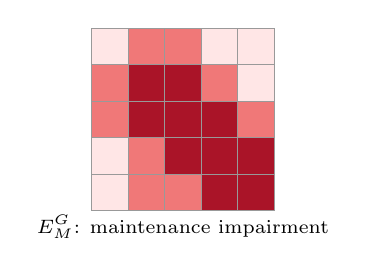
\begin{tikzpicture}[scale=0.58]
\cellbox{lowred}{(0,0)} \cellbox{midred}{(0.8,0)} \cellbox{midred}{(1.6,0)} \cellbox{highred}{(2.4,0)} \cellbox{highred}{(3.2,0)}
\cellbox{lowred}{(0,0.8)} \cellbox{midred}{(0.8,0.8)} \cellbox{highred}{(1.6,0.8)} \cellbox{highred}{(2.4,0.8)} \cellbox{highred}{(3.2,0.8)}
\cellbox{midred}{(0,1.6)} \cellbox{highred}{(0.8,1.6)} \cellbox{highred}{(1.6,1.6)} \cellbox{highred}{(2.4,1.6)} \cellbox{midred}{(3.2,1.6)}
\cellbox{midred}{(0,2.4)} \cellbox{highred}{(0.8,2.4)} \cellbox{highred}{(1.6,2.4)} \cellbox{midred}{(2.4,2.4)} \cellbox{lowred}{(3.2,2.4)}
\cellbox{lowred}{(0,3.2)} \cellbox{midred}{(0.8,3.2)} \cellbox{midred}{(1.6,3.2)} \cellbox{lowred}{(2.4,3.2)} \cellbox{lowred}{(3.2,3.2)}
\gridframe\rastlabel{$E_{M}^{G}$: maintenance impairment}
\end{tikzpicture}}

\newcommand{\drawRasterFeature}{%
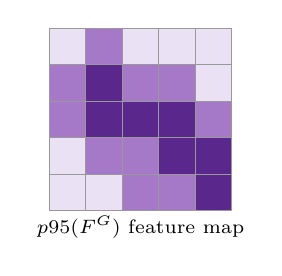
\begin{tikzpicture}[scale=0.58]
\cellbox{purpleA}{(0,0)} \cellbox{purpleA}{(0.8,0)} \cellbox{purpleB}{(1.6,0)} \cellbox{purpleB}{(2.4,0)} \cellbox{purpleC}{(3.2,0)}
\cellbox{purpleA}{(0,0.8)} \cellbox{purpleB}{(0.8,0.8)} \cellbox{purpleB}{(1.6,0.8)} \cellbox{purpleC}{(2.4,0.8)} \cellbox{purpleC}{(3.2,0.8)}
\cellbox{purpleB}{(0,1.6)} \cellbox{purpleC}{(0.8,1.6)} \cellbox{purpleC}{(1.6,1.6)} \cellbox{purpleC}{(2.4,1.6)} \cellbox{purpleB}{(3.2,1.6)}
\cellbox{purpleB}{(0,2.4)} \cellbox{purpleC}{(0.8,2.4)} \cellbox{purpleB}{(1.6,2.4)} \cellbox{purpleB}{(2.4,2.4)} \cellbox{purpleA}{(3.2,2.4)}
\cellbox{purpleA}{(0,3.2)} \cellbox{purpleB}{(0.8,3.2)} \cellbox{purpleA}{(1.6,3.2)} \cellbox{purpleA}{(2.4,3.2)} \cellbox{purpleA}{(3.2,3.2)}
\gridframe\rastlabel{$p95(F^G)$ feature map}
\end{tikzpicture}}

\newcommand{\drawClusterRaster}{%
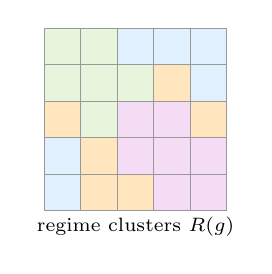
\begin{tikzpicture}[scale=0.58]
\cellbox{clusterone}{(0,0)} \cellbox{clustertwo}{(0.8,0)} \cellbox{clustertwo}{(1.6,0)} \cellbox{clusterfour}{(2.4,0)} \cellbox{clusterfour}{(3.2,0)}
\cellbox{clusterone}{(0,0.8)} \cellbox{clustertwo}{(0.8,0.8)} \cellbox{clusterfour}{(1.6,0.8)} \cellbox{clusterfour}{(2.4,0.8)} \cellbox{clusterfour}{(3.2,0.8)}
\cellbox{clustertwo}{(0,1.6)} \cellbox{clusterthree}{(0.8,1.6)} \cellbox{clusterfour}{(1.6,1.6)} \cellbox{clusterfour}{(2.4,1.6)} \cellbox{clustertwo}{(3.2,1.6)}
\cellbox{clusterthree}{(0,2.4)} \cellbox{clusterthree}{(0.8,2.4)} \cellbox{clusterthree}{(1.6,2.4)} \cellbox{clustertwo}{(2.4,2.4)} \cellbox{clusterone}{(3.2,2.4)}
\cellbox{clusterthree}{(0,3.2)} \cellbox{clusterthree}{(0.8,3.2)} \cellbox{clusterone}{(1.6,3.2)} \cellbox{clusterone}{(2.4,3.2)} \cellbox{clusterone}{(3.2,3.2)}
\gridframe\rastlabel{regime clusters $R(g)$}
\end{tikzpicture}}

\title{Synthetic Walkthrough of Threshold-Free Spatial Vulnerability Regime Analysis}
\author{TwoTimescaleResilience technical mock-up}
\date{\today}

\begin{document}
\maketitle

\section{Purpose}
This document is a synthetic visual mock-up of the proposed four-stage spatial vulnerability workflow:
\begin{enumerate}[label=Step \arabic*:,leftmargin=2.5cm]
\item threshold-free feature-vector construction;
\item standardisation and feature dropping;
\item clustering into vulnerability regimes;
\item maps, NetCDF, and raster integration.
\end{enumerate}
The example uses tiny rasters drawn directly in \LaTeX. The values are illustrative, but the mathematical objects match the intended TwoTimescaleResilience workflow.

\section{Starting Point: Concentration Rasters}
For compound $j$, month $t$, and grid cell $g=(x,y)$, let $C_{j,t}(g)$ be the ambient concentration. In a gridded workflow this is a stack of rasters:
\begin{equation}
\mathbf{C}_{j,t}\in\mathbb{R}^{n_y\times n_x}_{\ge 0}.
\end{equation}
For illustration, three compounds have distinct spatial patterns: a river/plume, diffuse runoff, and an urban hotspot.

\begin{center}
\begin{tabular}{ccc}
\drawRasterCOne & \drawRasterCTwo & \drawRasterCThree\\
\end{tabular}
\end{center}

These rasters are not clustered directly. They are first transformed through the model chain:
\begin{equation}
C_{j,t}(g)\rightarrow B_{j,t}(g)\rightarrow x_{j,t}(g)\rightarrow E_{a,t}^{(m)}(g)\rightarrow Q_{q,t}^{(m)}(g)\rightarrow A_{q,t}^{(m)}(g)\rightarrow \lambda_{q,t}^{(m)}(g)\rightarrow F_{q,t}^{(m)}(g).
\end{equation}

\section{Model Transformations}
Chemical memory is represented as
\begin{equation}
B_{j,t}(g)=\rho_j B_{j,t-1}(g)+(1-\rho_j)K_jC_{j,t}(g).
\end{equation}
Active stress is then
\begin{equation}
x_{j,t}(g)=\max\left(0,\frac{B_{j,t}(g)-\mathrm{NOEC}_j}{\mathrm{EC50}_j-\mathrm{NOEC}_j}\right).
\end{equation}
The stress is routed to a DEB-informed axis $a\in\{A,M,G,R\}$: assimilation, maintenance, growth, reproduction.

For the grouped CA-then-IA mixture model, within an axis and effect-code group $u$,
\begin{equation}
X_{a,u,t}(g)=\sum_{j:r(j)=a,\,h(j)=u}x_{j,a,t}(g),\qquad
E_{a,u,t}(g)=\frac{X_{a,u,t}(g)}{1+X_{a,u,t}(g)}.
\end{equation}
Across effect-code groups,
\begin{equation}
E_{a,t}^{G}(g)=1-\prod_u\left(1-E_{a,u,t}(g)\right).
\end{equation}
For a species or archetype $q$,
\begin{equation}
Q_{q,t}^{G}(g)=\sum_a w_{q,a}E_{a,t}^{G}(g),
\end{equation}
\begin{equation}
A_{q,t}^{G}(g)=A_{0,q}\max(10^{-6},1-Q_{q,t}^{G}(g)),
\end{equation}
and
\begin{equation}
F_{q,t}^{G}(g)=\frac{\lambda_q(A_{0,q})}{\lambda_q(A_{q,t}^{G}(g))}.
\end{equation}

\section{Step 1: Threshold-Free Feature Vector}
The feature-vector layer converts model outputs into one row per grid cell. It deliberately avoids fixed exceedance thresholds such as $F>1.10$ or $Q>0.80$. Instead it uses continuous summaries.

Example feature families are:
\begin{align}
&\text{Q features: } \overline{Q}^{G},\ Q_{0.50}^{G},\ Q_{0.90}^{G},\ Q_{0.95}^{G},\ Q_{\max}^{G},\ \mathrm{sd}(Q^G),\\
&\text{F features: } \overline{F}^{G},\ F_{0.50}^{G},\ F_{0.90}^{G},\ F_{0.95}^{G},\ F_{\max}^{G},\ \mathrm{sd}(F^G),\\
&\text{relative margin: } \overline{A/A_0},\ (A/A_0)_{0.50},\ (A/A_0)_{0.05},\ \min(A/A_0),\\
&\text{axis composition: } \overline{E}_A^G,\overline{E}_M^G,\overline{E}_G^G,\overline{E}_R^G,\ H_E,\\
&\text{mixture sensitivity: } \Delta F_{IA-TU},\ \Delta F_{G-TU},\ \Delta Q_{IA-TU},\ \Delta Q_{G-TU},\\
&\text{seasonal timing: } t^*_{F_{0.95}},\ t^*_{Q_{0.95}},\ t^*_{\sum_a E_a}.
\end{align}

Axis entropy is defined by
\begin{equation}
H_E(g)=-\sum_a p_a(g)\log p_a(g),\qquad
p_a(g)=\frac{\overline{E}_a^G(g)}{\sum_{a'}\overline{E}_{a'}^G(g)}.
\end{equation}
Low entropy means one axis dominates; high entropy means impairment is spread across axes.

\begin{center}
\begin{tabular}{cc}
\drawRasterAxis & \drawRasterFeature\\
\end{tabular}
\end{center}

A schematic feature matrix is:
\begin{center}
\small
\begin{tabular}{rrrrrrrr}
\toprule
cell & $x$ & $y$ & $p95(F^G)$ & $p95(Q^G)$ & $H_E$ & $\Delta F_{G-TU}$ & $t^*_F$\\
\midrule
1 & 1 & 1 & 1.01 & 0.08 & 0.05 & 0.00 & 3\\
2 & 2 & 1 & 1.06 & 0.21 & 0.10 & 0.01 & 4\\
3 & 3 & 1 & 1.19 & 0.45 & 0.44 & 0.05 & 7\\
4 & 4 & 1 & 1.42 & 0.72 & 0.31 & 0.13 & 8\\
5 & 5 & 1 & 1.51 & 0.78 & 0.25 & 0.18 & 8\\
\bottomrule
\end{tabular}
\end{center}

\section{Step 2: Standardisation and Feature Dropping}
Features have different units and scales. Before clustering, numeric features are standardised:
\begin{equation}
\widetilde{Z}_{g,p}=\frac{Z_{g,p}-\mu_p}{\sigma_p}.
\end{equation}
Stage 2 also drops unusable features:
\begin{itemize}
\item non-finite feature columns;
\item zero or near-zero variance columns;
\item optionally, highly correlated redundant features.
\end{itemize}
No new vulnerability features are created in this stage.

\begin{center}
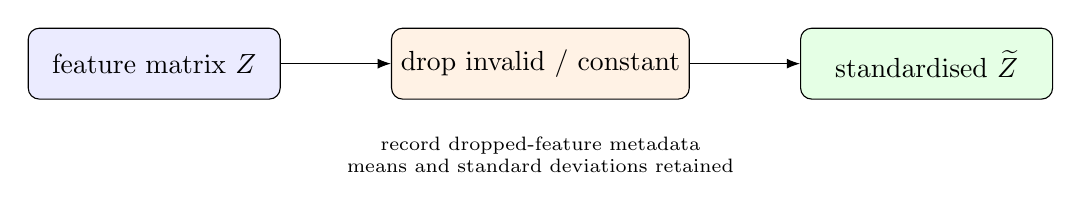
\begin{tikzpicture}[node distance=1.4cm,>=Latex]
\node[draw,rounded corners,fill=blue!8,minimum width=3.2cm,minimum height=0.9cm] (raw) {feature matrix $Z$};
\node[draw,rounded corners,fill=orange!10,right=of raw,minimum width=3.5cm,minimum height=0.9cm] (drop) {drop invalid / constant};
\node[draw,rounded corners,fill=green!10,right=of drop,minimum width=3.2cm,minimum height=0.9cm] (std) {standardised $\widetilde Z$};
\draw[->] (raw) -- (drop);
\draw[->] (drop) -- (std);
\node[below=0.35cm of drop,align=center,font=\scriptsize] {record dropped-feature metadata\\means and standard deviations retained};
\end{tikzpicture}
\end{center}

Example dropped-feature report:
\begin{center}
\small
\begin{tabular}{lll}
\toprule
feature & reason & detail\\
\midrule
mean\_E\_assimilation\_grouped & zero\_or\_near\_zero\_variance & all cells zero\\
month\_of\_max\_p95\_Q\_grouped & zero\_or\_near\_zero\_variance & all cells peak in month 8\\
max\_relative\_delta\_F\_grouped\_minus\_IA & high\_correlation & correlated with absolute delta\\
\bottomrule
\end{tabular}
\end{center}

\section{Step 3: Clustering}
Clustering is performed on the standardised continuous features, not on raw concentrations and not on threshold exceedance counts. A simple implementation can use deterministic $K$-means:
\begin{equation}
\min_{\mathcal{C}_1,\ldots,\mathcal{C}_K}\sum_{k=1}^{K}\sum_{g\in\mathcal{C}_k}\left\|\widetilde{\bm z}(g)-\bm\mu_k\right\|_2^2.
\end{equation}
The output is a regime label
\begin{equation}
R(g)\in\{1,\ldots,K\}.
\end{equation}

A synthetic cluster map might look like:
\begin{center}
\drawClusterRaster
\end{center}

Regimes should be named by their centroid characteristics, not by arbitrary thresholds:
\begin{center}
\small
\begin{tabular}{lll}
\toprule
cluster & suggested label & defining continuous features\\
\midrule
1 & low-response regime & low $p95(F^G)$, low $p95(Q^G)$, low axis impairment\\
2 & maintenance-dominated regime & high $\overline{E}_M^G$, low $H_E$\\
3 & multi-axis impairment regime & elevated $H_E$, moderate-to-high $Q_{0.95}^G$\\
4 & mixture-sensitive upper-envelope regime & high $F_{0.95}^G$, high $\Delta F_{G-TU}$\\
\bottomrule
\end{tabular}
\end{center}

\section{Step 4: Maps, NetCDF, and Raster Integration}
After clustering is stable, the workflow can write outputs as rasters or NetCDF variables. The core variables would be:
\begin{align}
&\texttt{cluster\_id[x,y]},\\
&\texttt{p95\_F\_grouped[x,y]},\quad \texttt{p95\_Q\_grouped[x,y]},\\
&\texttt{axis\_entropy[x,y]},\quad \texttt{dominant\_axis\_code[x,y]},\\
&\texttt{max\_delta\_F\_grouped\_minus\_TU[x,y]},\\
&\texttt{month\_of\_max\_p95\_F\_grouped[x,y]}.
\end{align}

\begin{center}
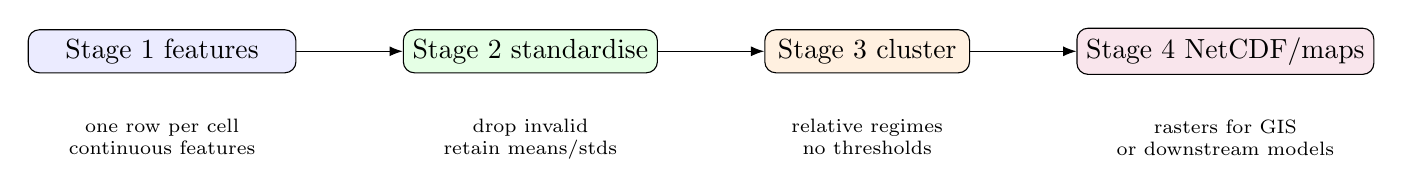
\begin{tikzpicture}[node distance=1.35cm,>=Latex]
\node[draw,rounded corners,fill=blue!8,minimum width=3.4cm] (features) {Stage 1 features};
\node[draw,rounded corners,fill=green!10,right=of features,minimum width=3.2cm] (std) {Stage 2 standardise};
\node[draw,rounded corners,fill=orange!12,right=of std,minimum width=2.6cm] (clus) {Stage 3 cluster};
\node[draw,rounded corners,fill=purple!10,right=of clus,minimum width=3.4cm] (netcdf) {Stage 4 NetCDF/maps};
\draw[->] (features) -- (std);
\draw[->] (std) -- (clus);
\draw[->] (clus) -- (netcdf);
\node[below=0.45cm of features,font=\scriptsize,align=center] {one row per cell\\continuous features};
\node[below=0.45cm of std,font=\scriptsize,align=center] {drop invalid\\retain means/stds};
\node[below=0.45cm of clus,font=\scriptsize,align=center] {relative regimes\\no thresholds};
\node[below=0.45cm of netcdf,font=\scriptsize,align=center] {rasters for GIS\\or downstream models};
\end{tikzpicture}
\end{center}

A future NetCDF schema could be:
\begin{center}
\small
\begin{tabular}{lll}
\toprule
variable & dimensions & meaning\\
\midrule
\texttt{cluster\_id} & \texttt{x,y} & vulnerability regime label\\
\texttt{p95\_F\_grouped} & \texttt{x,y} & upper-envelope amplification feature\\
\texttt{axis\_entropy} & \texttt{x,y} & spread of impairment across DEB axes\\
\texttt{dominant\_axis\_code} & \texttt{x,y} & 0 none, 1 assimilation, 2 maintenance, 3 growth, 4 reproduction\\
\texttt{max\_delta\_F\_G\_minus\_TU} & \texttt{x,y} & mixture-effect sensitivity\\
\texttt{month\_of\_max\_p95\_F} & \texttt{x,y} & seasonal timing of upper-envelope response\\
\bottomrule
\end{tabular}
\end{center}

\section{What to Expect}
The final product is not a wall of heatmaps for many species. Instead, the expected outputs are:
\begin{enumerate}
\item a threshold-free feature matrix with one row per grid cell;
\item a standardised feature matrix suitable for clustering;
\item a vulnerability-regime map;
\item centroid summaries explaining the regimes;
\item continuous feature rasters for interpretation;
\item NetCDF outputs ready for GIS or further raster workflows.
\end{enumerate}

The key scientific constraint is that vulnerability regimes are derived from continuous model geometry: $E_a$, $Q$, $A/A_0$, $F$, axis entropy, seasonal timing, and mixture-model deltas. They are not defined by arbitrary exceedance thresholds.

\end{document}
